% !TEX root = main.tex
\section{Experiments and Results}
\label{sec:results}
\comment{

\begin{table}[t]
    \begin{center}
    \setlength{\tabcolsep}{1.3mm}
\begin{tabular}{r|cccccccccc}
\hline
& {\bf PDIA } & PDIA-MAP &  HMM-EM & bigram& trigram & 4-gram & 5-gram & 6-gram & SSM \\
\hline
AIWS & 2.36 & 2.45 &  2.98 & 3.28 & 2.69 & 2.36 & 2.26 & 2.23 & 2.26 \\
AIWS & 373.3 & 379 & 52 & 28 & 382 & 2023 & 5592 & 10,838 & 19,358 \\
\hline
\hline
AIWL & 2.03 & 2.05 &  2.98 & 3.24 & 2.52& 2.02 & 1.81 & 1.73 & 1.70 \\
AIWL & 1,231.6 & 1,247 &  52 & 28 & 444 & 3,249 & 12,324 & 31,990 & 177,232 \\
\hline
\hline
DNA & 1.89 & 1.90 &  1.91 & 1.91 & 1.91 & 1.90 & 1.90 & 1.90 & 1.83 \\
DNA & 61.3 & 54 & 46.2* &  5 & 21 & 85 & 341 & 1,365 & 314,166 \\
\hline
\end{tabular}
\end{center}
\caption[Short]{Benchmark performance of PDIA inference algorithms versus standard sequence models.}
\label{table:results}
\end{table}


\begin{table}[t]
    \begin{center}
    \setlength{\tabcolsep}{1.3mm}
\begin{tabular}{r|cccccccccc}
\hline
& {\bf PDIA } & PDIA-MAP &  HMM & bigram& trigram & 4-gram & 5-gram & 6-gram & SSM \\
\hline
AIWS & 2.362 & 2.448 &  2.98 & 3.275 & 2.687 & 2.358 & 2.263 & 2.230 & 2.257 \\
AIWS & 373.3 & 379 & 52 & 28 & 382 & 2023 & 5592 & 10838 & 19358 \\
\hline
\hline
AIWL & 2.027 & 2.047 &  2.98 & ? & 2.517 & 2.018 & 1.811 & 1.729 & 1.697 \\
AIWL & 1231.6 & 1247 &  52 & 28 & 444 & 3249 & 12324 & 31990 & 177232 \\
\hline
\hline
DNA & 1.894 & 1.896 &  1.909 & 1.913 & 1.906 & 1.903 & 1.898 & 1.895 & 1.832 \\
DNA & 61.3 & 54 & 46.2* &  5 & 21 & 85 & 341 & 1365 & 314166 \\
\hline
\end{tabular}
\end{center}
\caption[Short]{Benchmark performance of PDIA inference algorithms versus standard sequence models.}
\label{table:results}
\end{table}
}


\begin{table}[t]
    \begin{center}
    \setlength{\tabcolsep}{1.3mm}
\begin{tabular}{r|cccccccccc}
\hline
& PDIA  & PDIA-MAP &  HMM-EM & bigram& trigram & 4-gram & 5-gram & 6-gram & SSM \\
\hline
AIW & 5.13 & 5.46 &  7.89 & 9.71 & 6.45 & 5.13 & 4.80 & 4.69 & 4.78 \\
  & 365.6 & 379 & 52 & 28 & 382 & 2023 & 5592 & 10,838 & 19,358 \\
\hline
\hline
%AIWL & 4.08 & 4.13 &  7.89 & 9.45 & 5.72 & 4.05 & 3.51 & 3.32 & 3.24 \\
 %AIWL & 1,231.6 & 1,247 &  52 & 28 & 444 & 3,249 & 12,324 & 31,990 & 177,232 \\
%\hline
%\hline
DNA & 3.72 & 3.72 &  3.76 & 3.77 & 3.75 & 3.74 & 3.73 & 3.72 & 3.56 \\
 & 61.3 & 54 & 46.2 &  5 & 21 & 85 & 341 & 1,365 & 314,166 \\
\hline
\end{tabular}
\end{center}
\caption[Short]{PDIA inference performance relative to known sequence models.  Top row: perplexity.  Bottom row: average number of states in the model.}
\label{table:results}
\end{table}

To test our PDIA inference approach we evaluated it on discrete natural sequence prediction and compared its performance against HMMs and smoothed n-gram models.  We trained the models on two datasets: a character sequence from Alice in Wonderland and a short sequence of mouse DNA.  The Alice in Wonderland dataset was preprocessed to remove all characters but letters and spaces, shift all letters from upper case to lower case, and split along sentence dividers to yield a 27-character alphabet (a-z and space)\comment{ and 1,639 sentences with a total of 132,794 characters.  We used the first 1,200 sentences (100,210 characters) to train the models and the rest to test}.  We trained on 100 random sentences (9,986 characters) and tested on 50 random sentences (3,891 characters).   The mouse DNA dataset consisted of a fragment of chromosome 2 with 194,173 base pairs, which we treated as a single unbroken string.  We used the first 150,000 base pairs for training and the rest for testing.  For Alice in Wonderland, the state of the PDIA model was always set to $q_0$ at the start of each sentence.  For DNA, the state of the PDIA model at the start of the test data was set to the last state of the model after accepting the training data.  We placed Gamma(1,1) priors over $\alpha$, $\beta$ and $\gamma$ and set $\lambda=.001.$

We evaluated the performance of the learned models by calculating the average per character predictive perplexity of the test data.  For training data $x_{1:T}$, test data $y_{1:T'}$ this is given by $2^{-\frac{1}{T'}\log_2\, P(y_{1:T'}|x_{1:T})}$.  It is an average measure of the uncertainty the model has about what character comes next in the sequence given the sequence up to that point, and is at most $|\Sigma|$.  We evaluated the probability of the test data incrementally, integrating test observations into the model in the standard Bayesian way\comment{, and averaged each predictive probability $P(y_{1:T'}|x_{1:T}) =  \prod_{i = 1}^{T'} \int P(y_i|y_{1:i-1},x_{1:T},\delta)P(\delta|y_{1:i-1},x_{1:T})d\delta \approx \frac{1}{L}\prod_{i = 1}^{T'} \sum_{\ell = 1}^{L} P(y_i|y_{1:i-1},x_{1:T},\delta_\ell)$ where $\delta_\ell \sim P(\delta|y_{1:i-1},x_{1:T})$}.  The asymptotic cost of prediction for the PDIA is $\mathcal{O}(LT')$, while for the HMM it is $\mathcal{O}(KT')$, where $K$ is the number of states.%In addition to averaging over multiple $\delta_\ell$, we also evaluated the log loss for each $\delta_\ell$ by itself to find the single model with the best generalization performance, which we call $\delta_{MAP}$.

Test perplexity results are shown in Table~\ref{table:results} on the first line of each of the AIW (Alice in Wonderland) and DNA (mouse DNA) subtables.  
For the smoothed $n$-gram models, we report thousand-sample average perplexity results for hierarchical Pitman-Yor process (HPYP) \cite{Teh2006a} models of varying Markov order (1 through 5 notated as bigram through 6-gram) after burning each model in for one hundred samples.  We also show the performance of the single particle incremental variant of the sequence memoizer (SM) \cite{Gasthaus2010}, the SM being the limit of an $n$-gram model as $n\rightarrow\infty$.
We also show results for a hidden Markov model (HMM) \cite{Murphy2005} trained using expectation-maximization (EM).  We determined the best number of hidden states by cross-validation on the test data (an procedure used here to produce optimistic HMM performance for comparison purposes only).  

%The log loss and optimal number of states are given in Table \ref{table:results}, and plots showing the generalization performance across a range of model sizes relative to PDIA performance is given in Figures \ref{fig:dna_hmm} and \ref{fig:aiw_small_hmm}.  

The performance of our PDIA learning approach exceeds that of the HMM and is approximately equal to that of a smoothed 4-gram model, it does not outperform very deep, smoothed Markov models.  Notably, it does easily outperform non-smoothed Markov models and outperforms the HDP-HMM 

 however, Table~\ref{table:results} also shows the number of states in each of the models (second line in both the AIW and DNA subtables).

While the PDIA averages over a  class of models that includes finite order Markov models as a subset, the states in HPYP are identifiable which means that hierarchical smoothing of the per-state emission distributions is possible.  In the PDIA model the states are not identifiable and no easily defined hierarchy of contextual specificity exists on which hierarchical smoothing can be implemented.   Note that the PDIA posterior average achieves


\begin{figure}[htbp]
\centering
\subfigure[DNA HMM EM Baseline]{\label{fig:dna_hmm}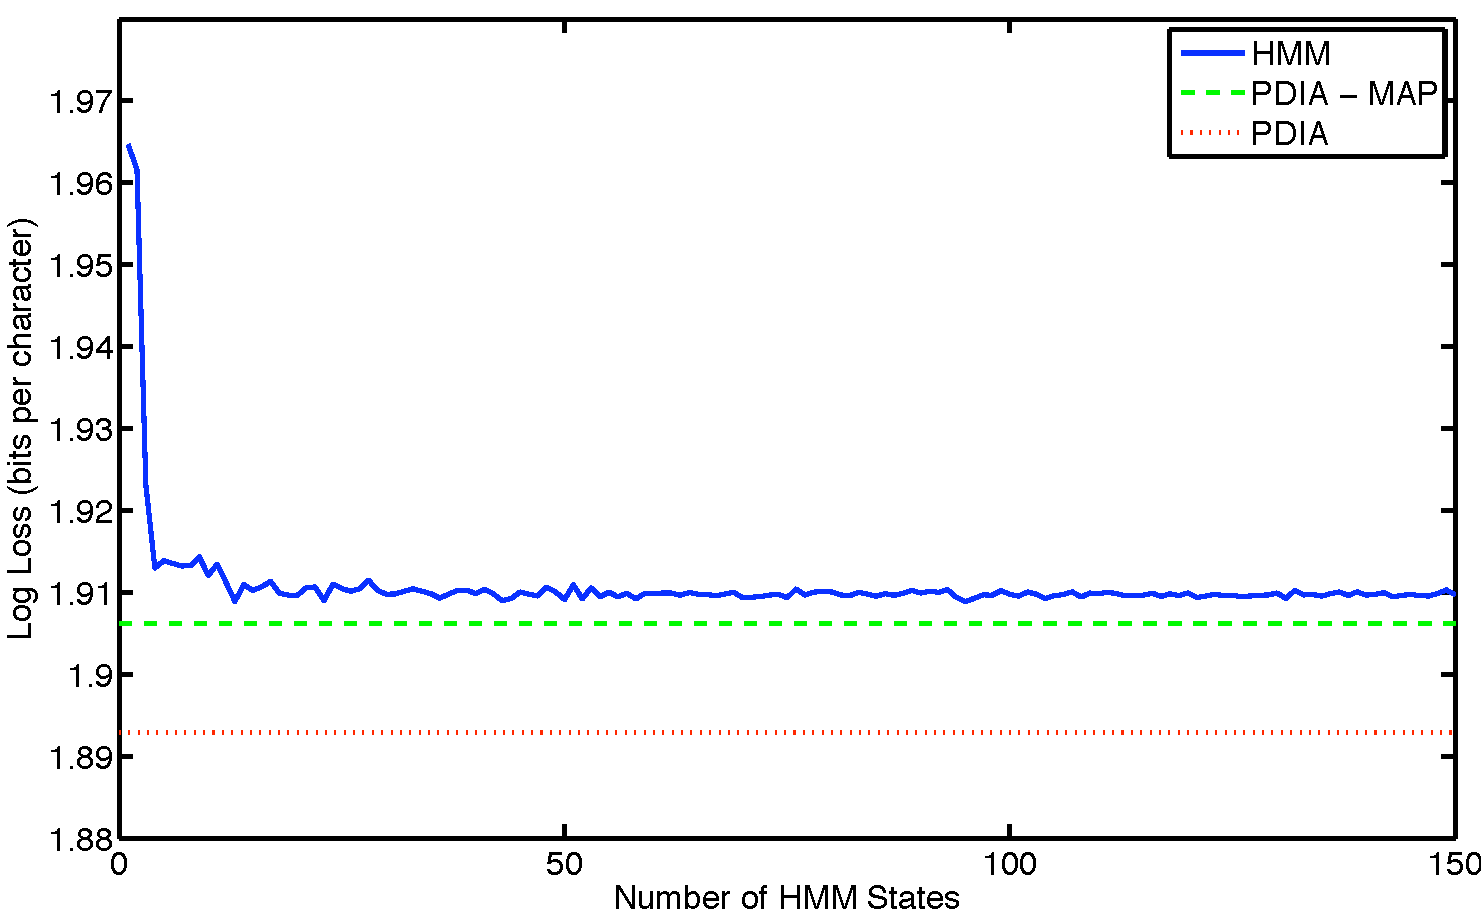
\includegraphics[width=.3\textwidth]{results/dna_hmm}}
\subfigure[DNA sampler trace]{\label{fig:dna_sampler}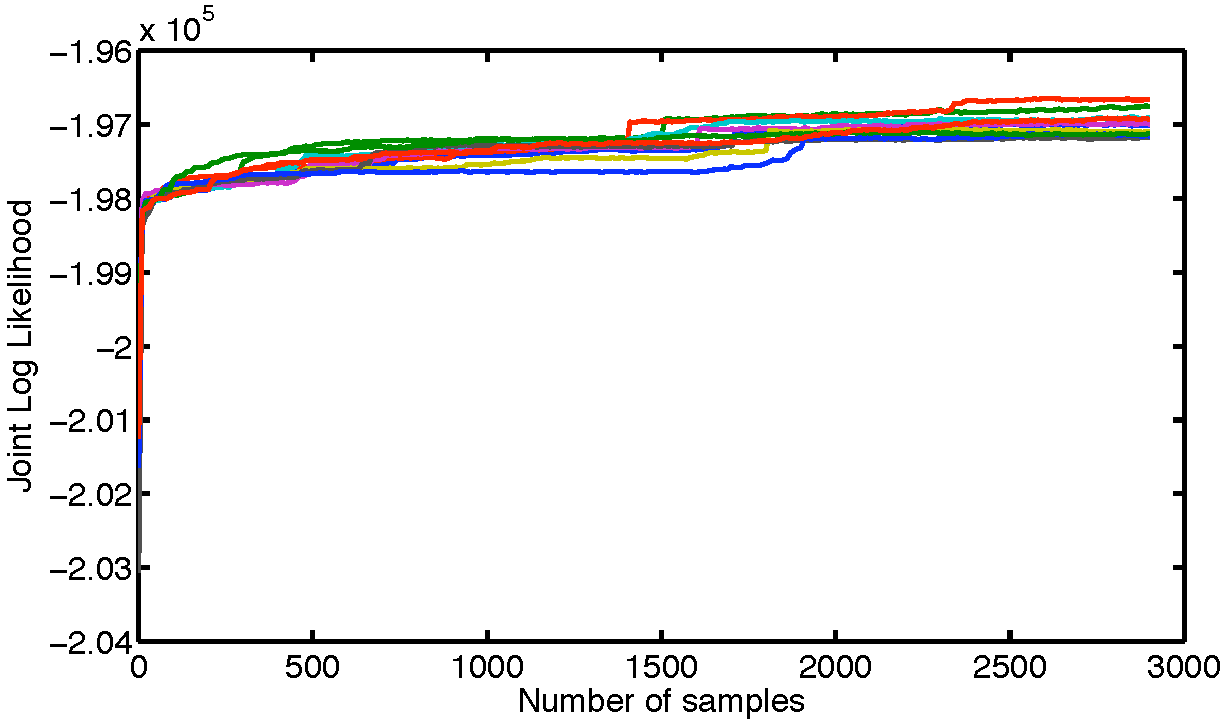
\includegraphics[width=.3\textwidth]{results/dna_sampler}}
\subfigure[DNA number of states]{\label{fig:dna_numstates}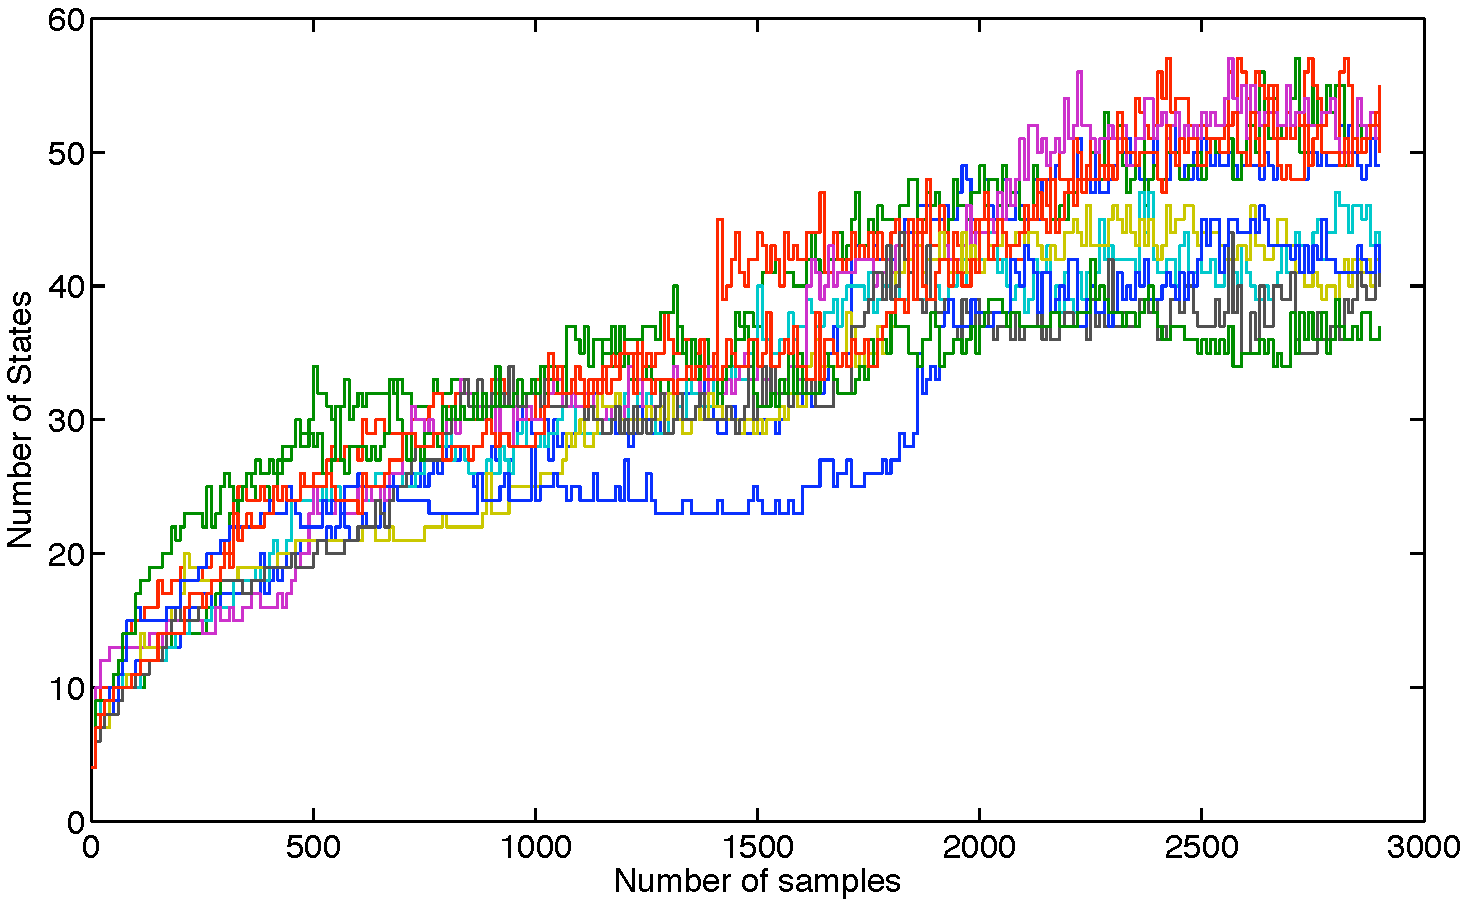
\includegraphics[width=.3\textwidth]{results/dna_numstates}}\\
\subfigure[AIW HMM EM Baseline]{\label{fig:aiw_small_hmm}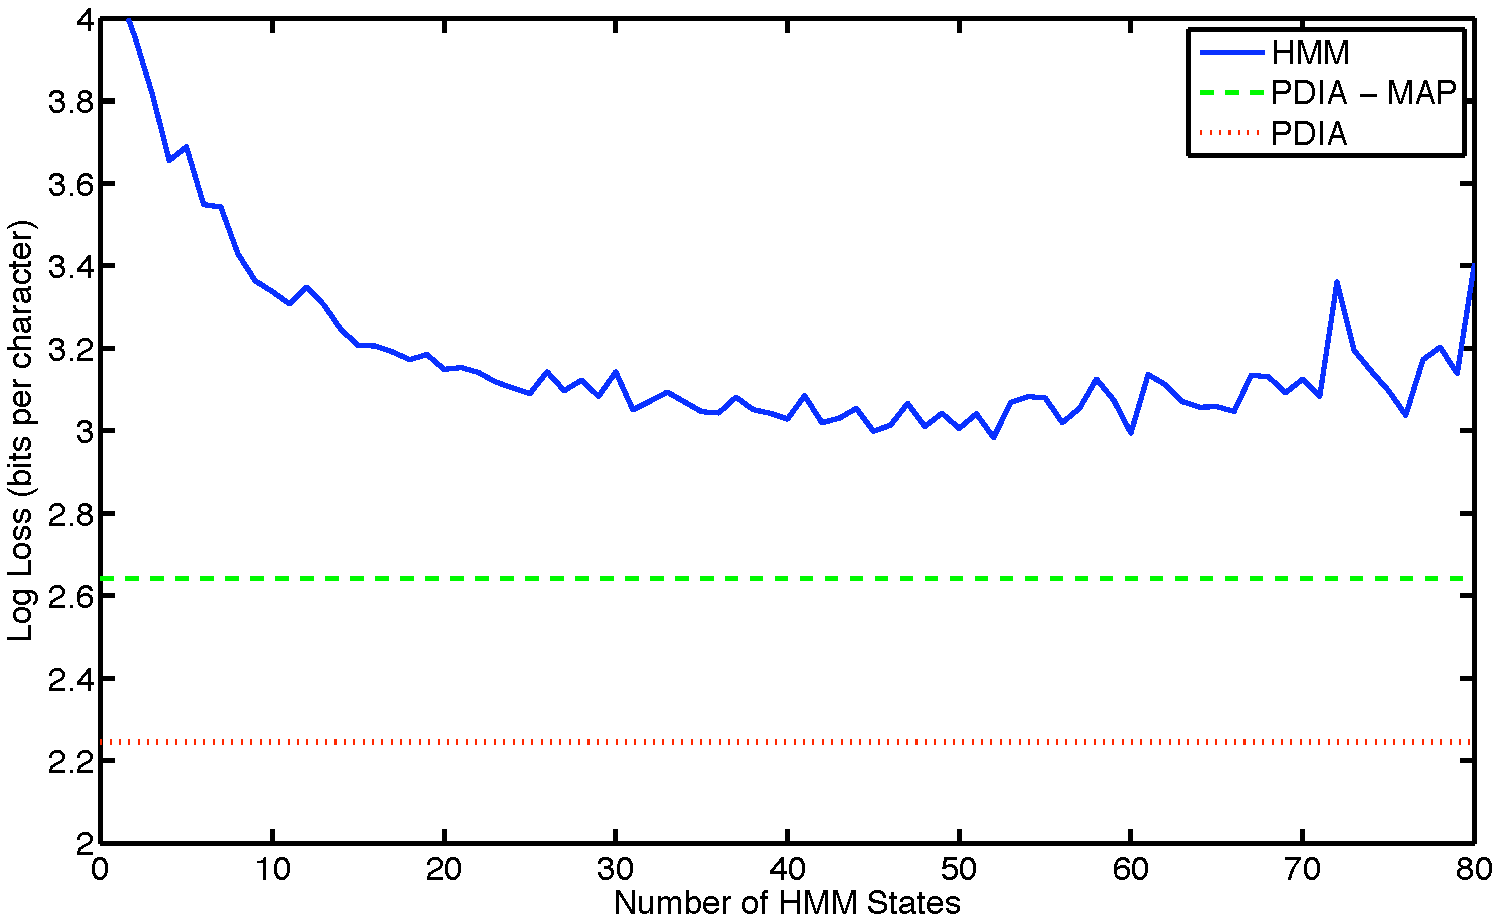
\includegraphics[width=.3\textwidth]{results/aiw_small_hmm}}
\subfigure[AIW sampler trace]{\label{fig:aiw_small_sampler}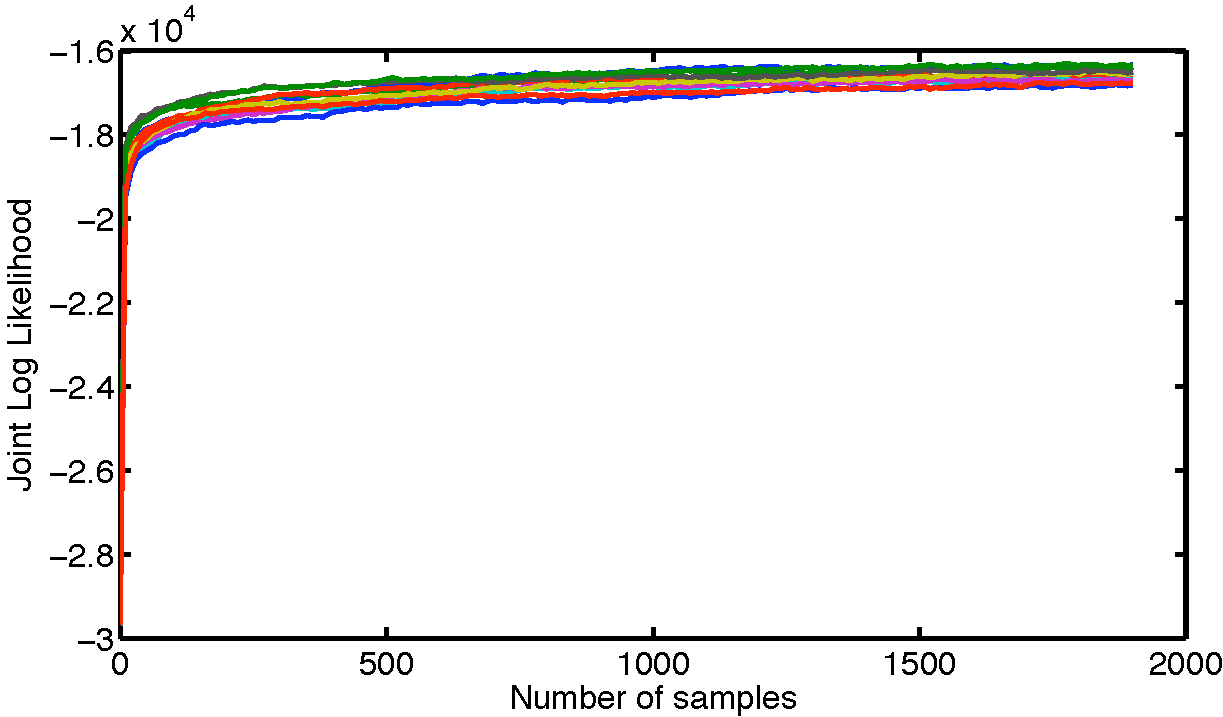
\includegraphics[width=.3\textwidth]{results/aiw_small_sampler}}
\subfigure[AIW number of states]{\label{fig:aiw_small_numstates}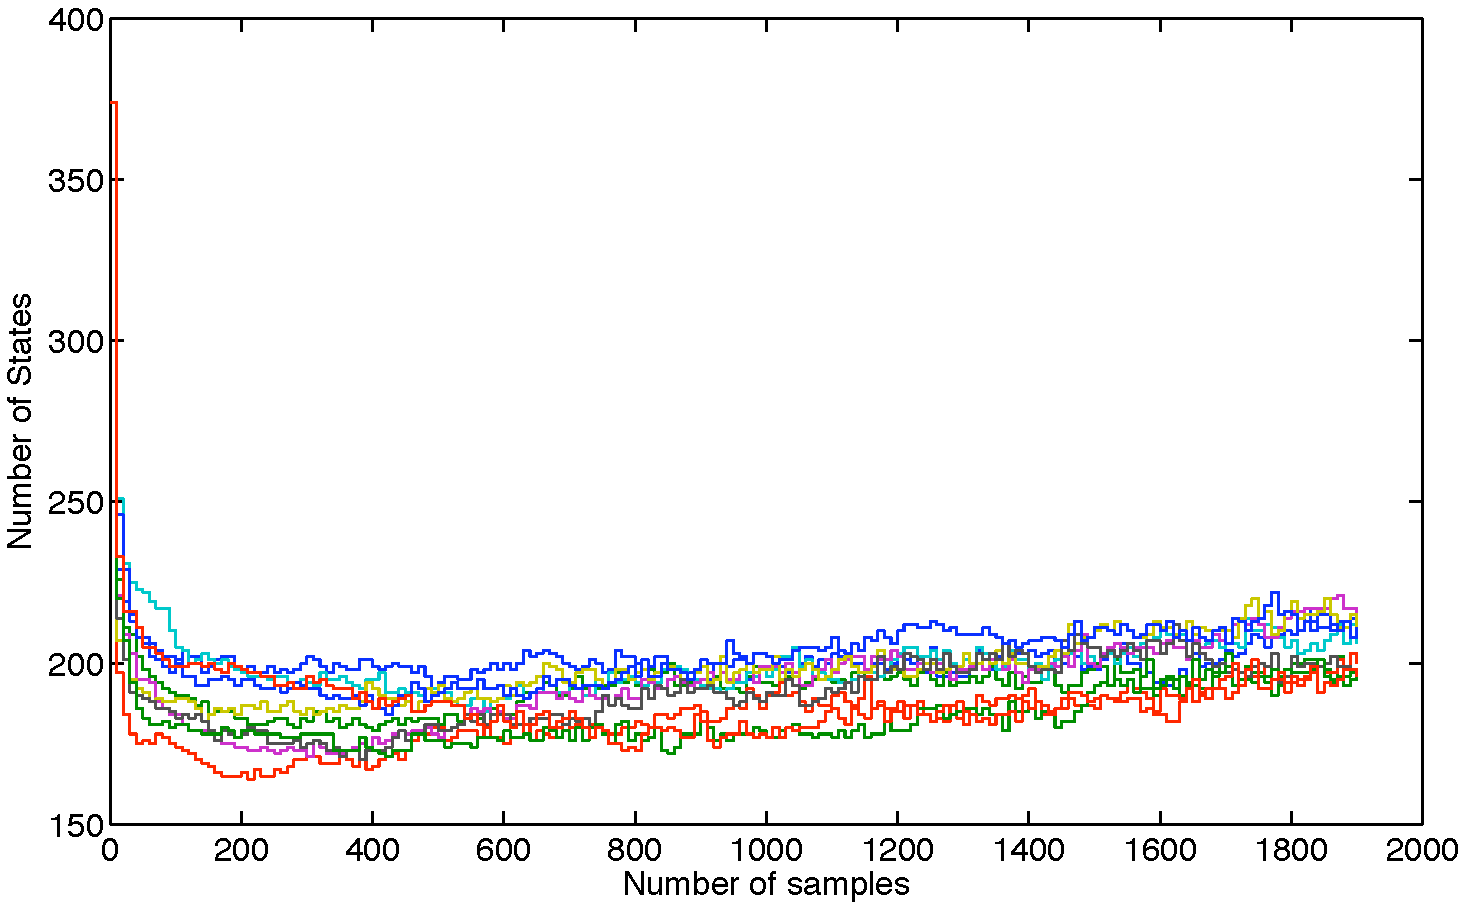
\includegraphics[width=.3\textwidth]{results/aiw_small_numstates}}
\caption{}
\label{fig:aiw_and_dna_all_figs}
\end{figure}





%We found that both the MAP PDIA and the average over PDIA generalize better than the HMM.  To test the possibility that better generalization was due to smoothing of the PDIA emission probability by $\beta$, we took samples from the PDIA, fixed $\beta$ to be very near 0, and ran the MCMC sampler as before.  We found that neither the average number of states nor the generalization performance was significantly affected.

%In general it seems that posterior samples from the PDIA achieve competitive generalization performance on natural language and DNA compared to hidden Markov models and n-gram models.  Averaging predictive probability over multiple samples leads to better generalization than a single sampled model.  Both a single sample and multiple samples generalize better than the best EM-trained HMM.  On natural language, the learned PDIA has more states than the optimal number of states for an HMM found by cross-validation.  The improved generalization is not due to smoothing the emission distribution.  Compared to smoothed n-gram models, the PDIA performs competitively even though there is no backing off to more general contexts.




%Even for a single sampled transition matrix $\delta_\ell$, there may be symbols $y_t$ which have not been emitted from the state $\q_t$ in the training data, and thus $\delta_\ell(\q_t,y_t)$ is not known.  In this case we sampled a new element of the transition matrix according to the CRF, as described in \ref{model}.  In the same way that we averaged the predictive probability of each character over multiple $\delta_\ell$, we averaged the probability of a character given a single $\delta_\ell$ over multiple sampled values of $\delta_\ell(\q_t,y_t)$.



